\documentclass{article}

\usepackage[utf8]{inputenc} % For Unicode characters
\usepackage{amsmath}        % For mathematical symbols
\usepackage{graphicx}       % For including images
\usepackage{hyperref}       % For hyperlinks
\usepackage{geometry}      % For setting page margins
\usepackage{float}
\usepackage{tcolorbox}

% Set the page margins
\geometry{margin=1in}
% Set the top margins
\addtolength{\topmargin}{-.5in}

\title{Engineering Optics, Homework 2}
\author{He Tianyang}
\date{\today}

\begin{document}

\maketitle

\section{Problem 1}
\textbf{Chapter 2, Problem 1}\\\\

\subsection{Positive Lens}

\begin{enumerate}
    \item $-\infty$, Image plane is at $f$.
          \begin{figure}[H]
              \centering
              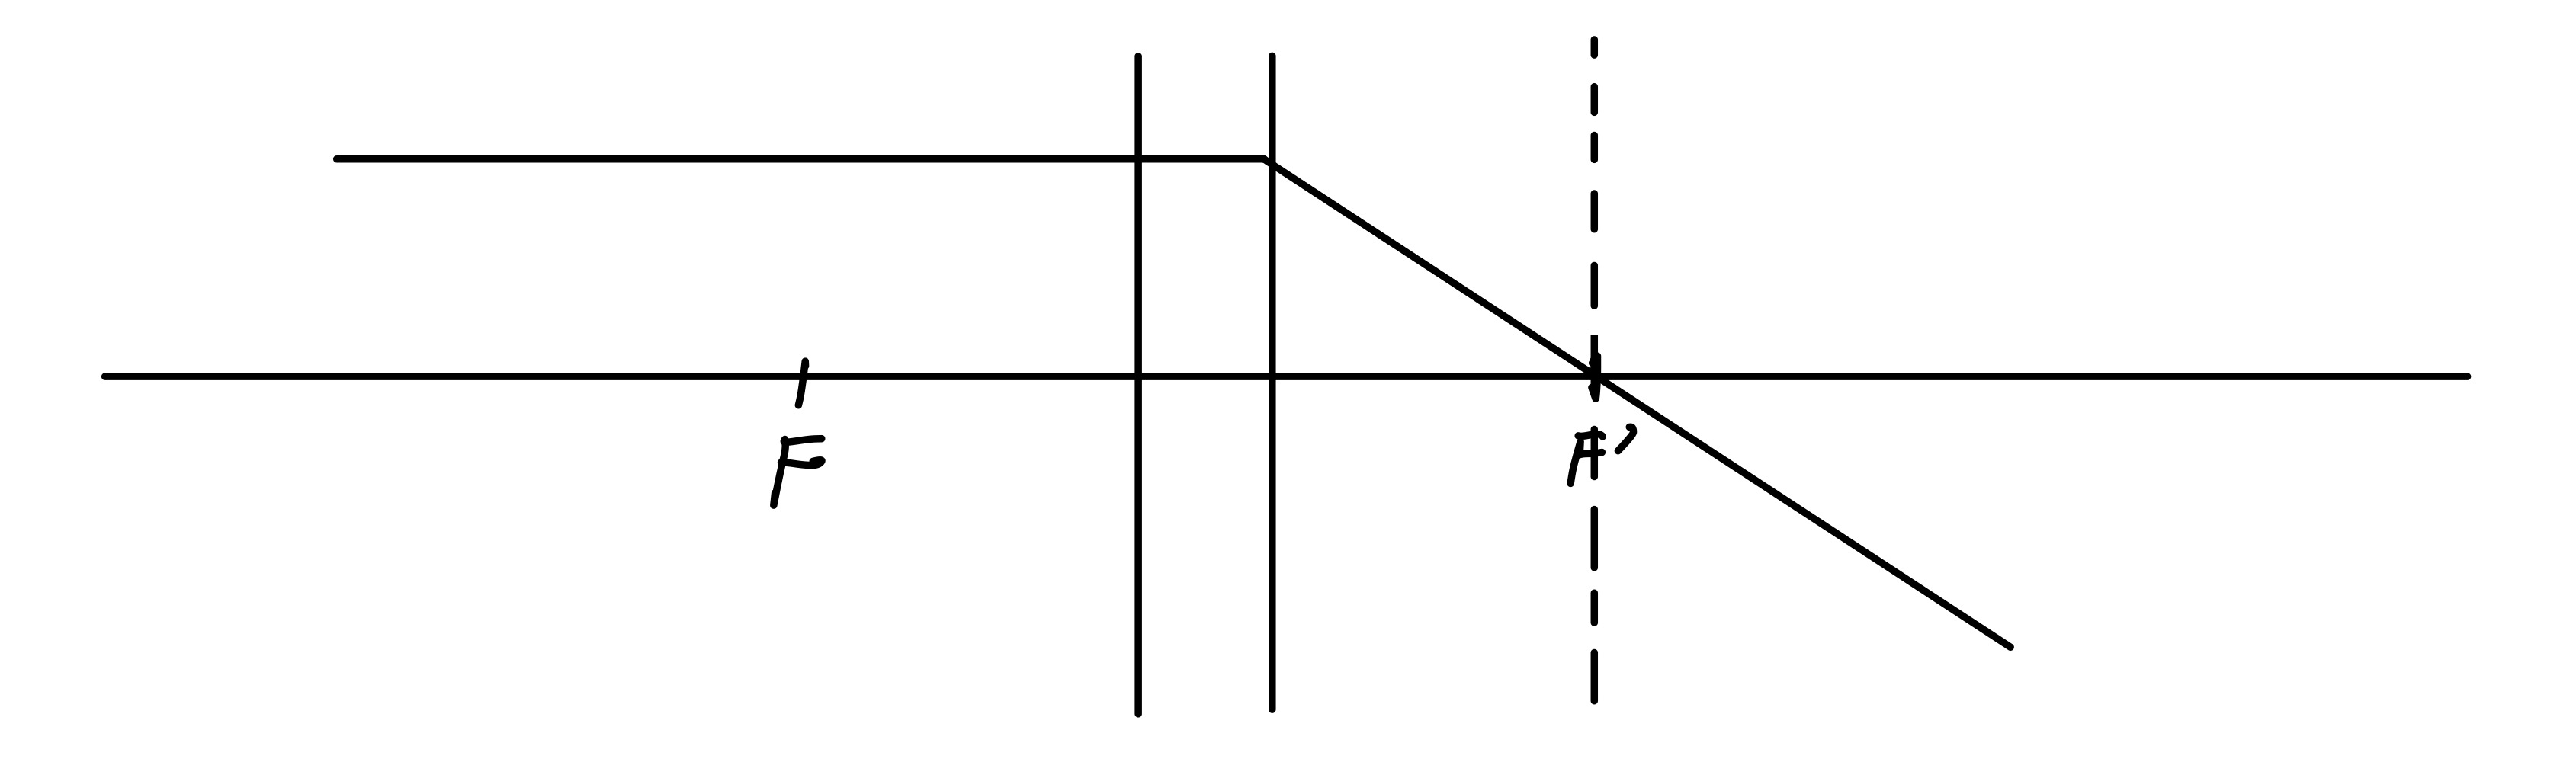
\includegraphics[width=0.5\textwidth]{image/hw2/hw2_1_1.jpeg}
              \caption{Object at $-\infty$}
          \end{figure}
    \item $-2f$, Image plane is at $2f$.
          \begin{figure}[H]
              \centering
              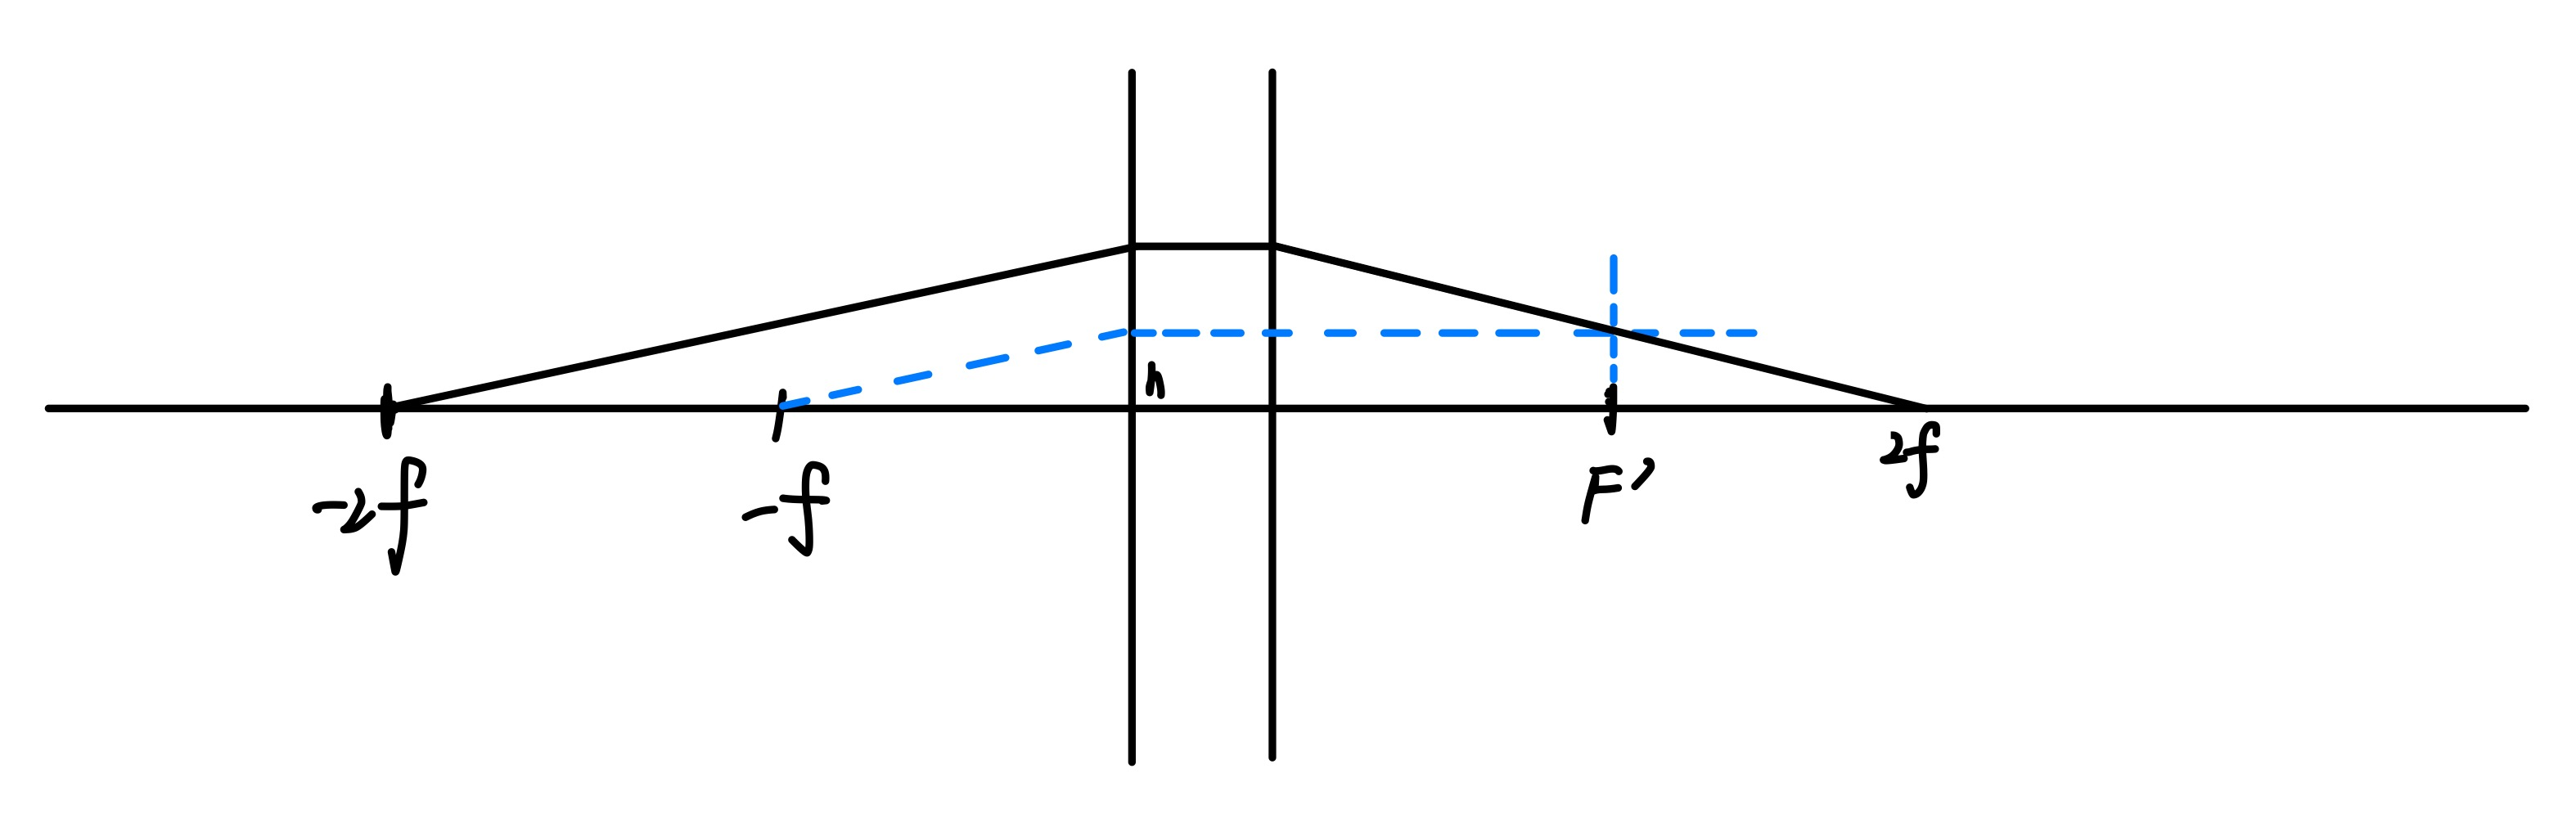
\includegraphics[width=0.5\textwidth]{image/hw2/hw2_1_2.jpeg}
              \caption{Object at $-2f$}
          \end{figure}
    \item $-f$, Image plane is at $\infty$.
          \begin{figure}[H]
              \centering
              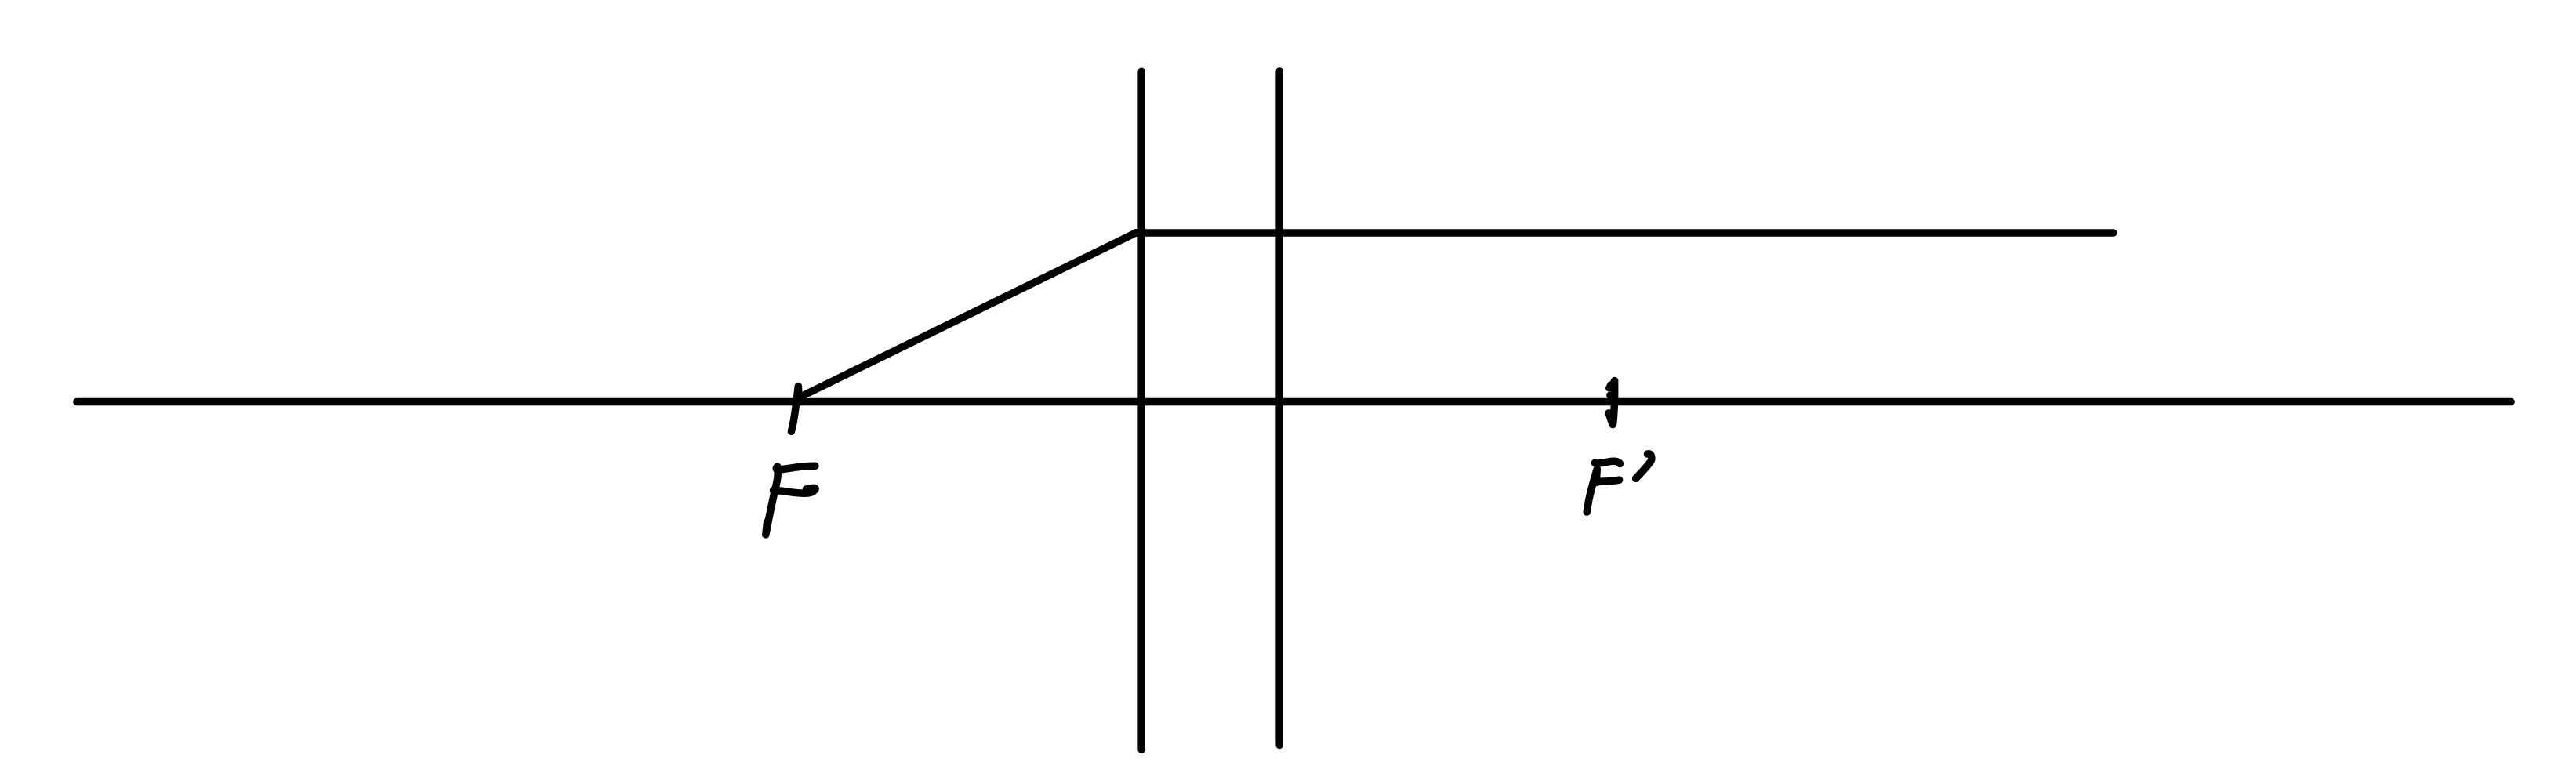
\includegraphics[width=0.5\textwidth]{image/hw2/hw2_1_3.jpeg}
              \caption{Object at $-f$}
          \end{figure}
    \item $-\frac{f}{2}$, Image plane is at $-f$.
          \begin{figure}[H]
              \centering
              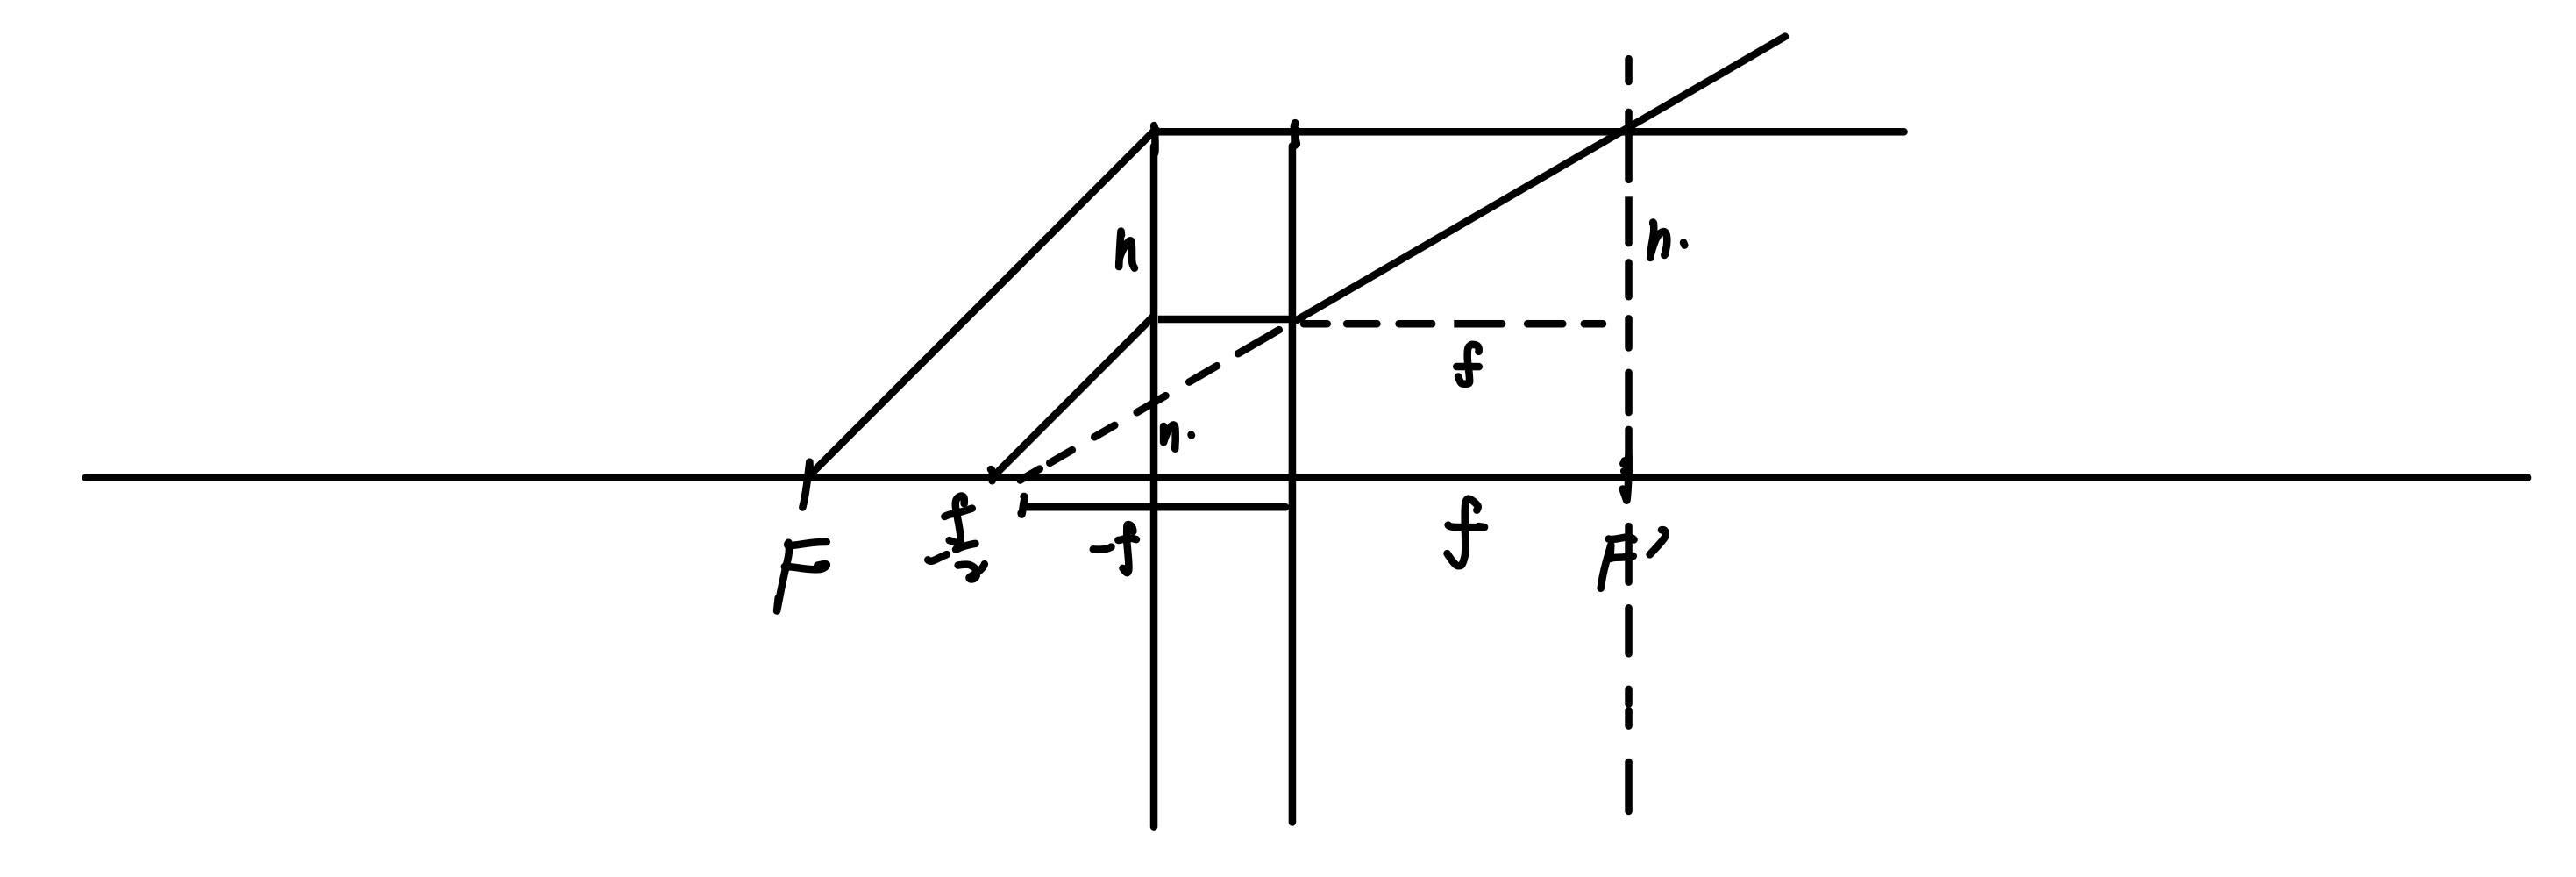
\includegraphics[width=0.5\textwidth]{image/hw2/hw2_1_4.jpeg}
              \caption{Object at $-0.5f$}
          \end{figure}
    \item $0$, Image plane is at $0$.
          \begin{figure}[H]
              \centering
              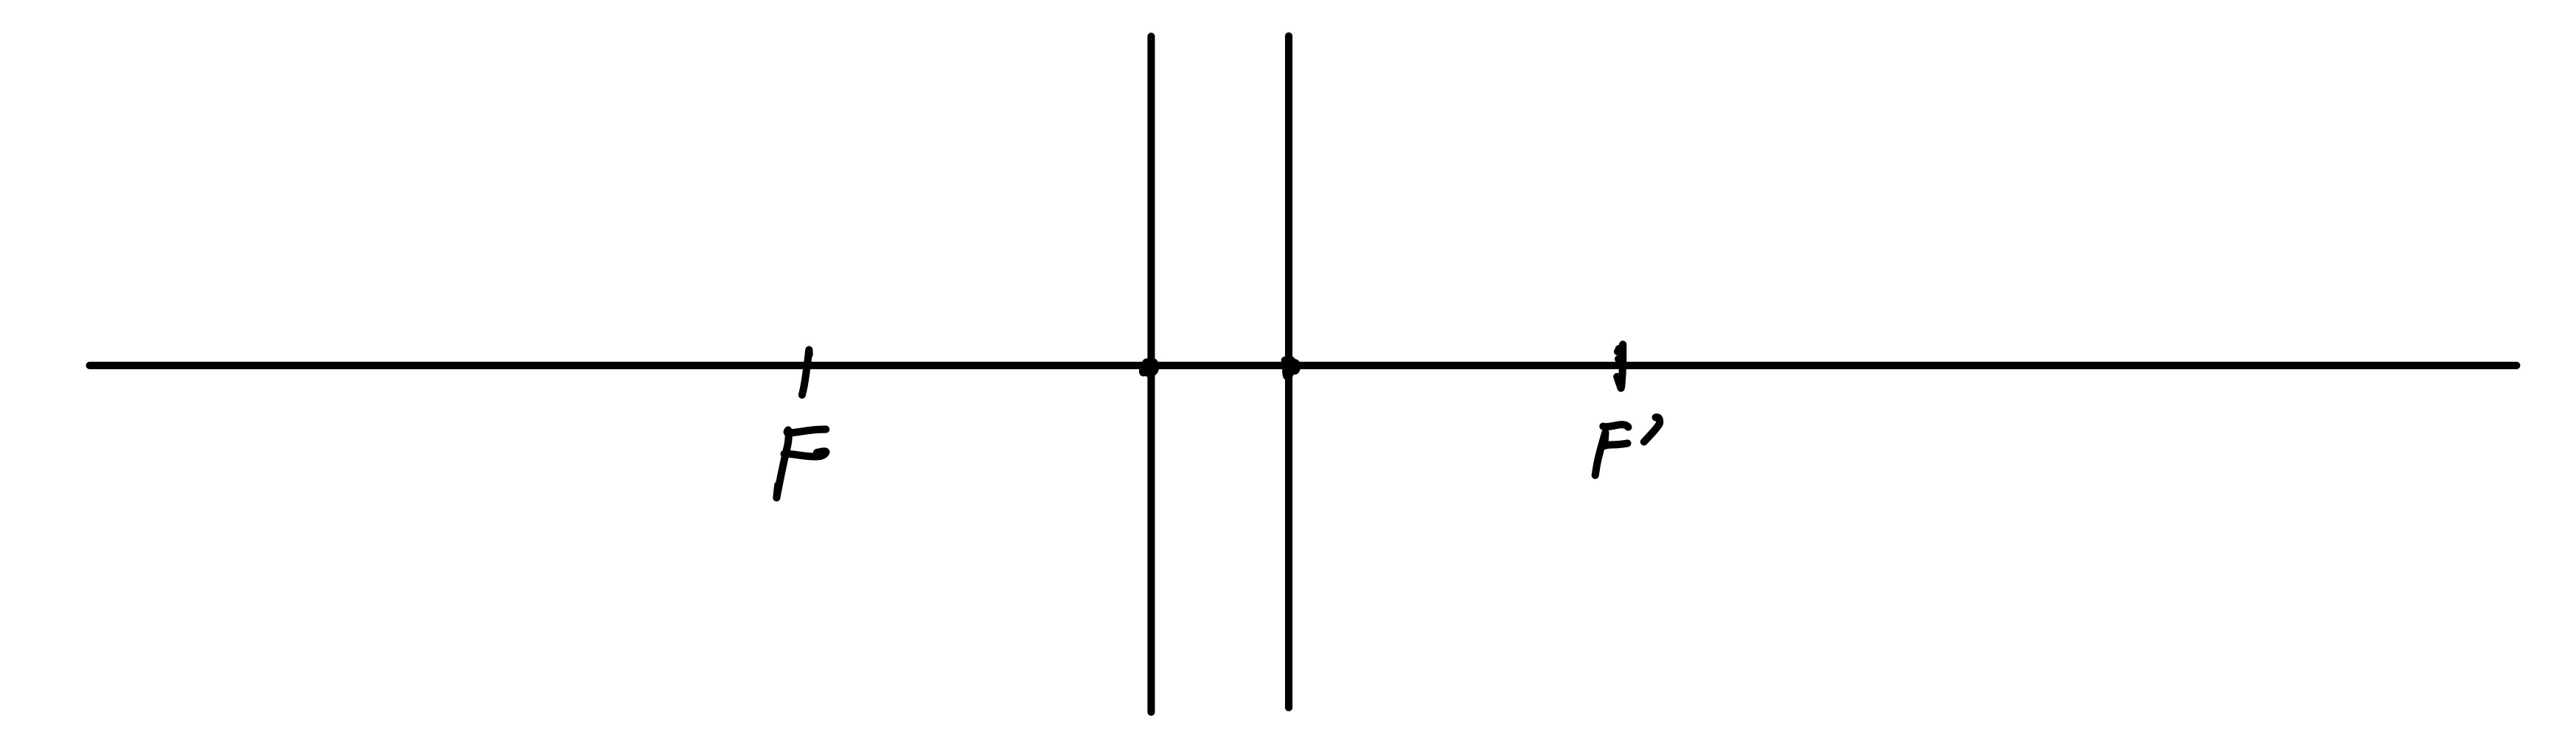
\includegraphics[width=0.5\textwidth]{image/hw2/hw2_1_5.jpeg}
              \caption{Object at $0$}
          \end{figure}
    \item $\frac{f}{2}$, Image plane is at $f$.
          \begin{figure}[H]
              \centering
              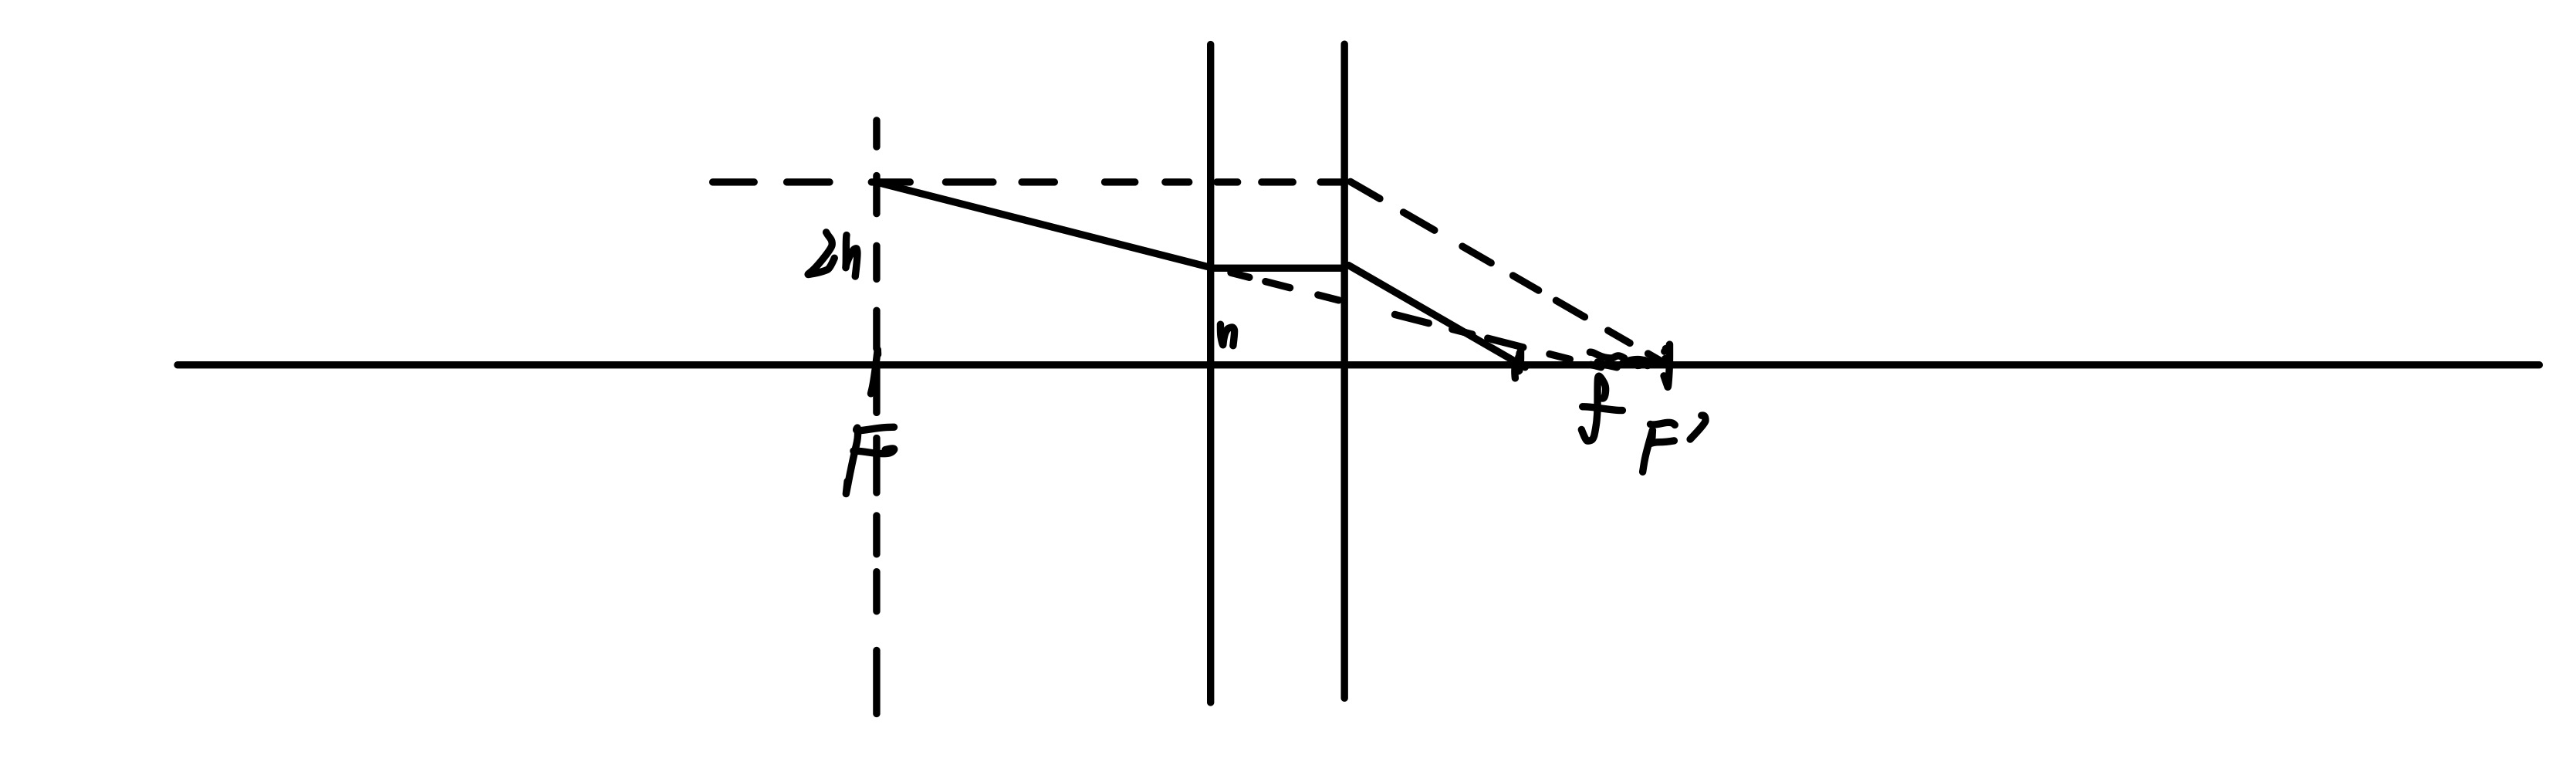
\includegraphics[width=0.5\textwidth]{image/hw2/hw2_1_6.jpeg}
              \caption{Object at $0.5f$}
          \end{figure}
    \item $f$, Image plane is at $-\infty$.
          \begin{figure}[H]
              \centering
              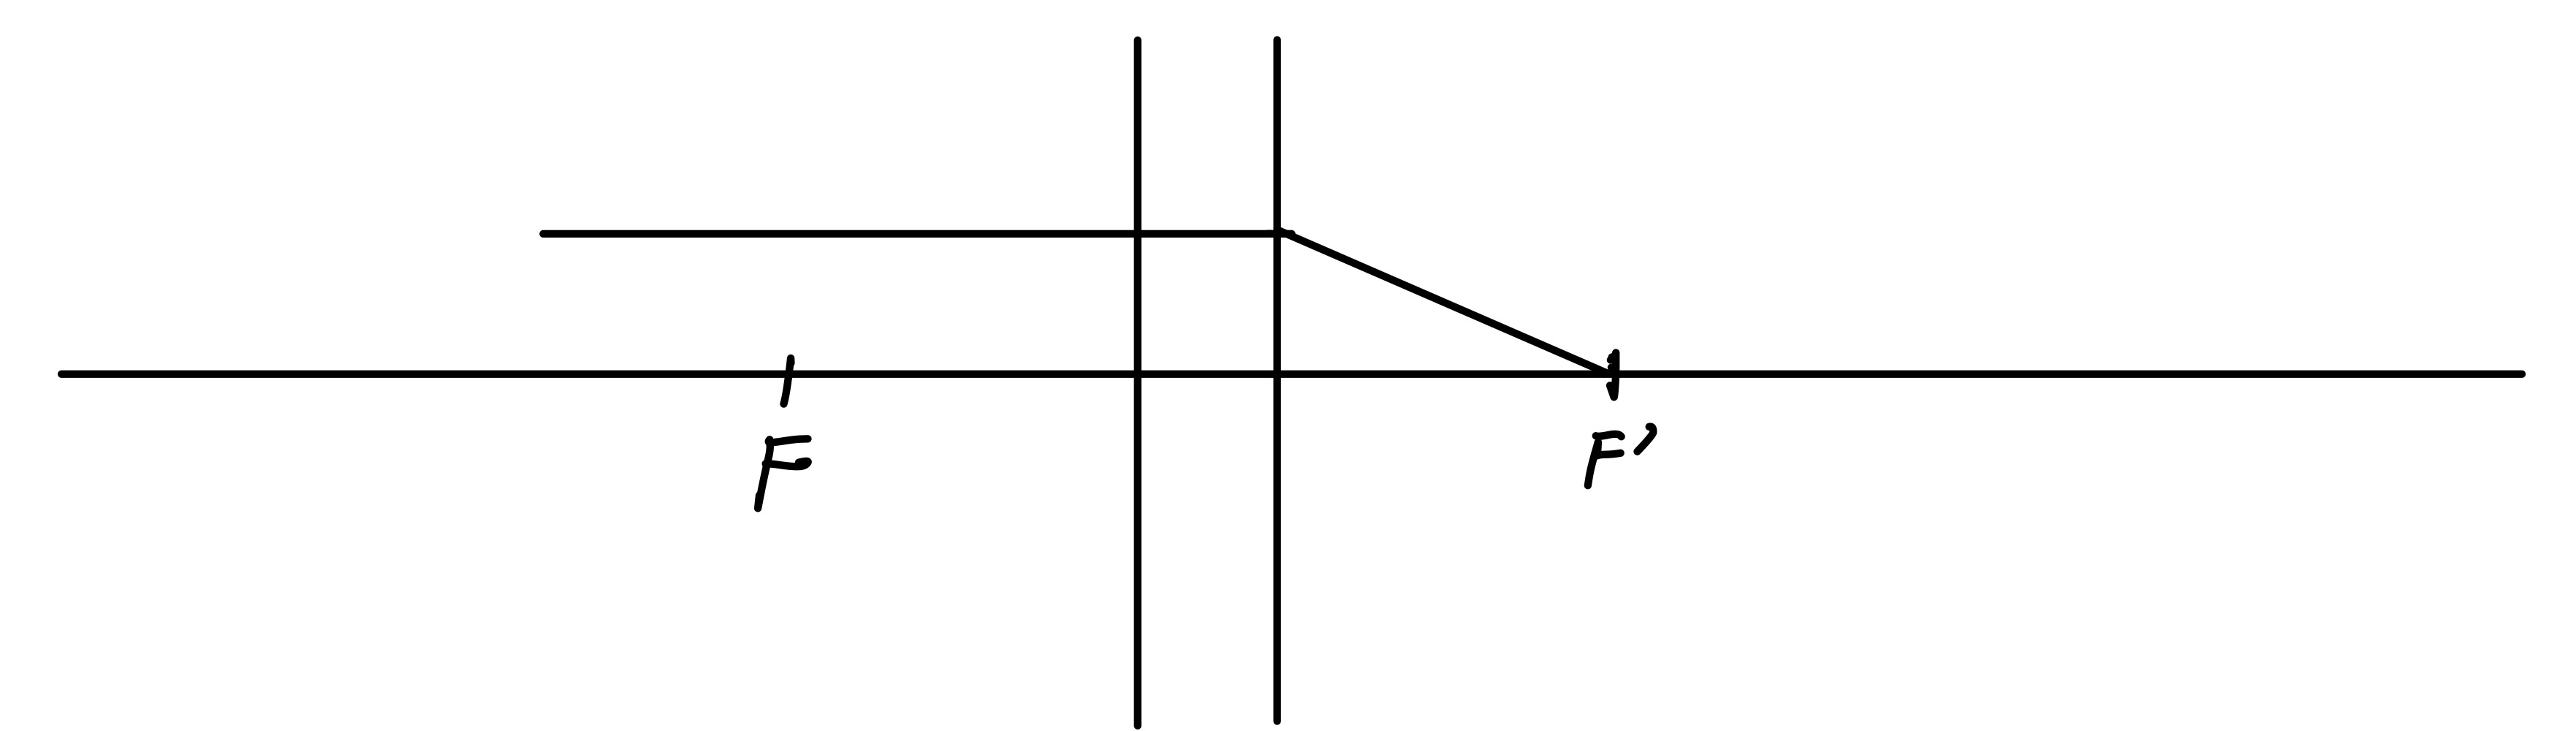
\includegraphics[width=0.5\textwidth]{image/hw2/hw2_1_7.jpeg}
              \caption{Object at $f$}
          \end{figure}
    \item $2f$, Image plane is at $-2f$.
          \begin{figure}[H]
              \centering
              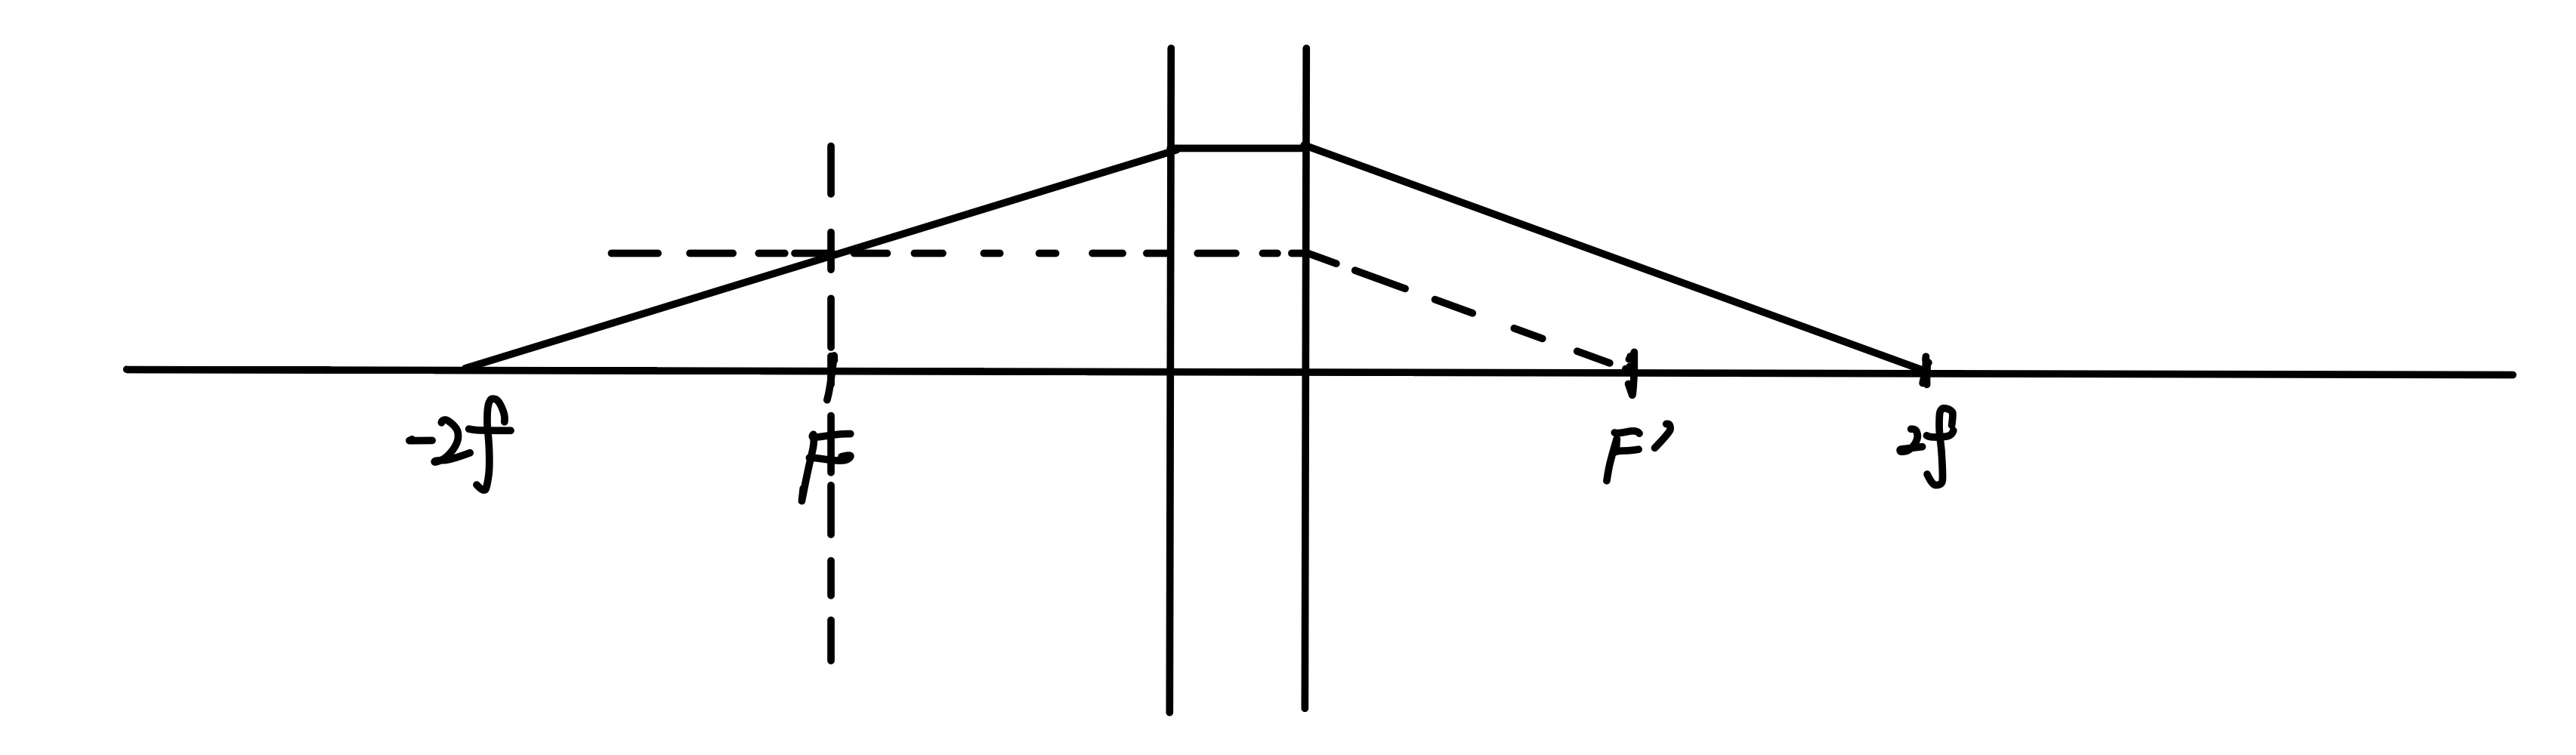
\includegraphics[width=0.5\textwidth]{image/hw2/hw2_1_8.jpeg}
              \caption{Object at $2f$}
          \end{figure}
    \item $+\infty$, Image plane is at $-f$.
          \begin{figure}[H]
              \centering
              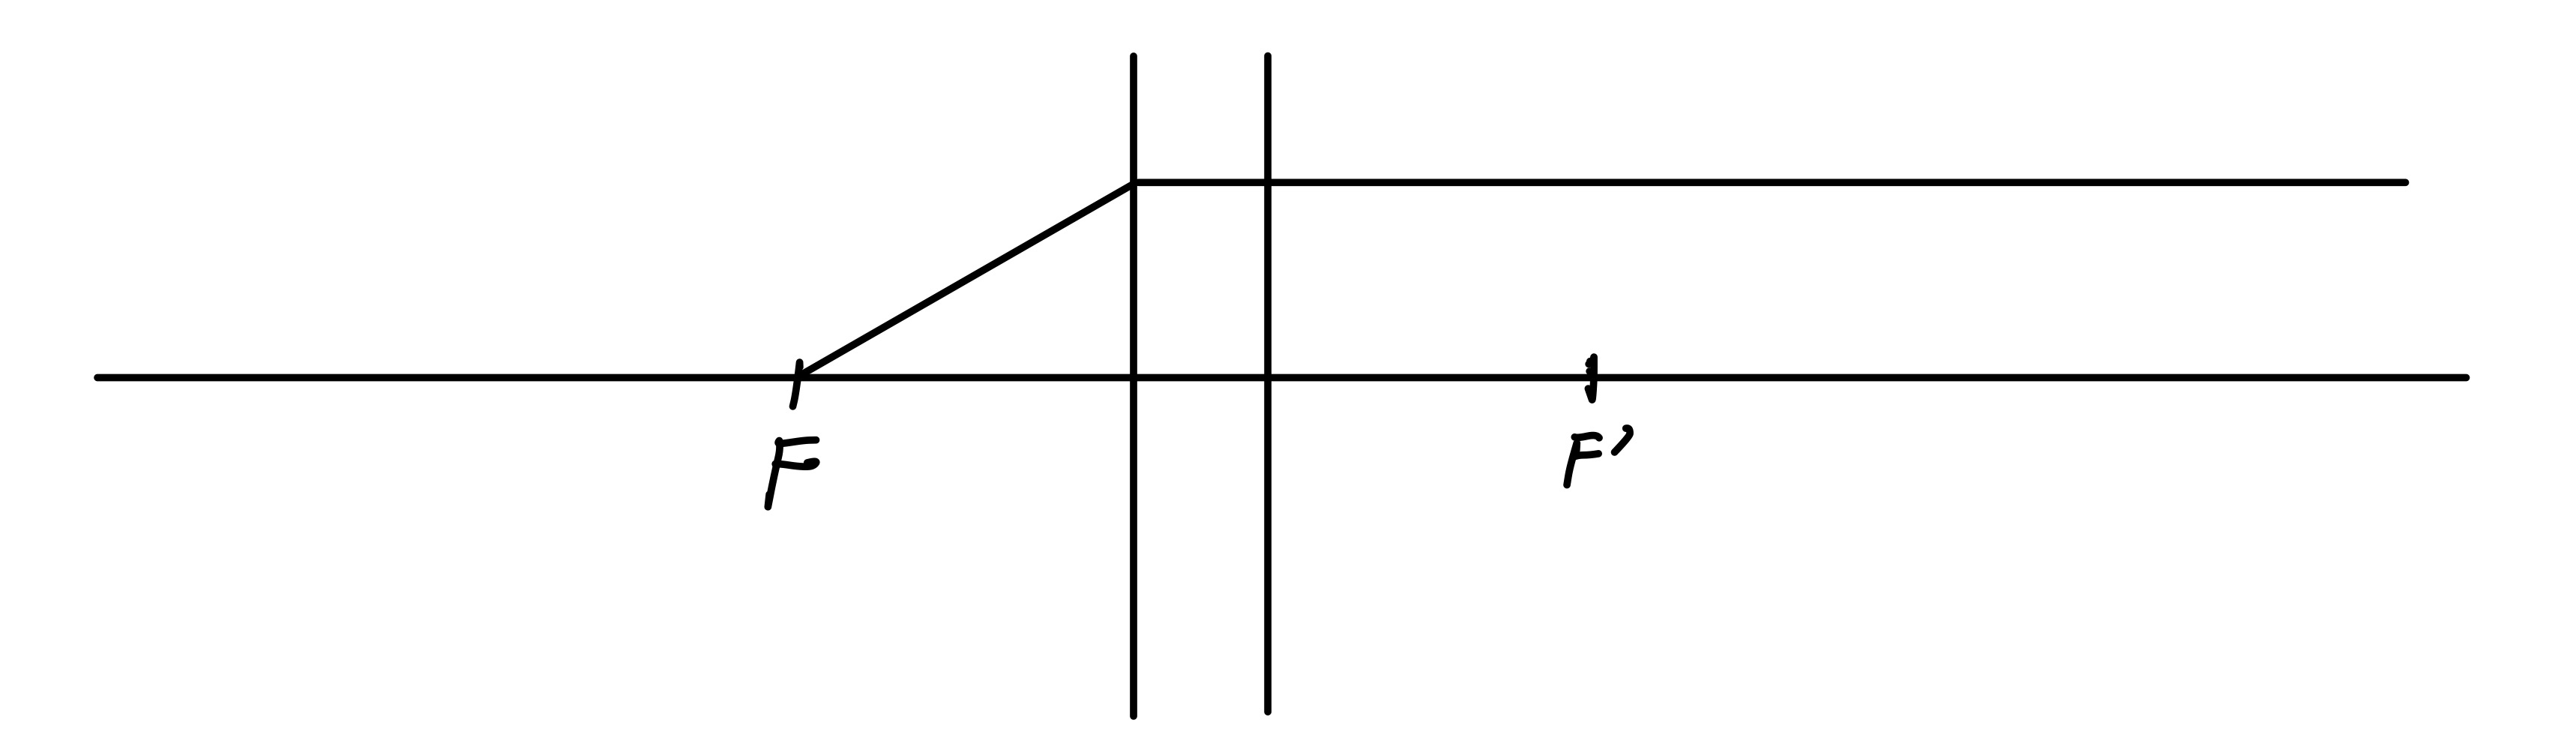
\includegraphics[width=0.5\textwidth]{image/hw2/hw2_1_9.jpeg}
              \caption{Object at $+\infty$}
          \end{figure}
\end{enumerate}

\section{Problem 2}
\textbf{Chapter 2, Problem 2}\\\\

Donated the $F$ as the zero point of the axis, we can use the Newtonian form of the lens equation to solve the problem. The lens equation is given by
\begin{equation}
    xx'=ff'
\end{equation}

Therefore, the Object at $-\infty, -10m, -8m, -6m, -4m, -2m$ follows the equation
\begin{align}
    x_1\cdot \infty & =f\cdot f' \\
    x_2\cdot 10     & =f\cdot f' \\
    x_3\cdot 8      & =f\cdot f' \\
    x_4\cdot 6      & =f\cdot f' \\
    x_5\cdot 4      & =f\cdot f' \\
    x_6\cdot 2      & =f\cdot f' \\
\end{align}

And
\begin{equation*}
    -f=f'= 75mm
\end{equation*}

Solving the equation, we can get the position of the image plane for each object plane. The result is shown in the table below.
\begin{align}
    x_1 & =\frac{ff'}{\infty} = 0mm                                                             \\
    x_2 & = \frac{ff'}{10} = \frac{5.625\times 10^{-3}}{10} = 5.625\times 10^{-4}m = 0.5625mm   \\
    x_3 & = \frac{ff'}{8} = \frac{5.625\times 10^{-3}}{8} = 7.03125\times 10^{-4}m = 0.703125mm \\
    x_4 & = \frac{ff'}{6} = \frac{5.625\times 10^{-3}}{6} = 9.375\times 10^{-4}m = 0.9375mm     \\
    x_5 & = \frac{ff'}{4} = \frac{5.625\times 10^{-3}}{4} = 1.40625\times 10^{-3}m = 1.40625mm  \\
    x_6 & = \frac{ff'}{2} = \frac{5.625\times 10^{-3}}{2} = 2.8125\times 10^{-3}m = 2.8125mm    \\
\end{align}

\section{Problem 3}
\textbf{Chapter 2, Problem 3}\\\\

\begin{figure}[H]
    \centering
    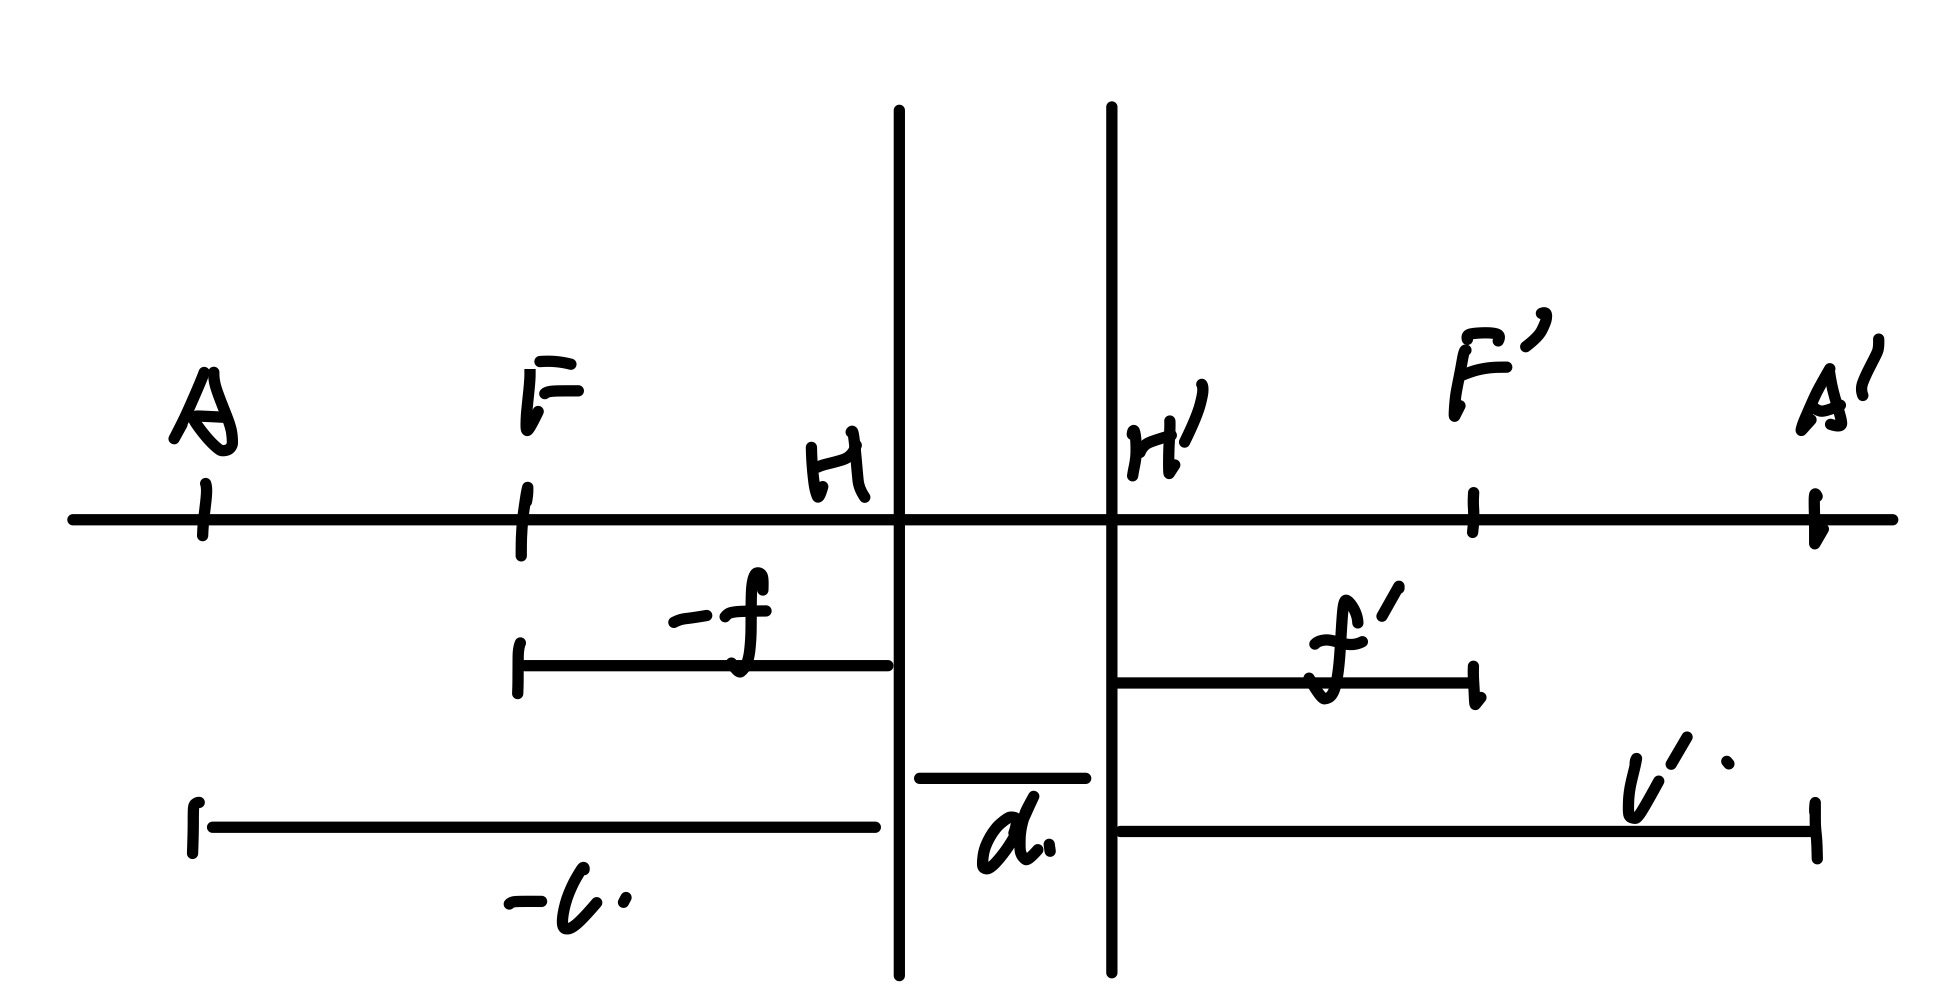
\includegraphics[width=0.5\textwidth]{image/hw2/hw2_2_1.jpeg}
    \caption{Optical System}
    \label{fig:optical_system}
\end{figure}

The Optical system is placed in the air, so we have
\begin{equation}
    n'=n,\quad -f=f'
\end{equation}

And assume the optical system is formed like Figure.\ref{fig:optical_system}, we can use the Newtonian form of the lens equation to solve the problem. The lens equation is given by
\begin{equation}
    \begin{cases}
        \beta = \frac{l'}{l} \\
        f'+(-f)+d = 1140     \\
        l'+(-l)+d=7200       \\
        \frac{1}{l'}-\frac{1}{l} = \frac{1}{f'}
    \end{cases}
\end{equation}

Solving the equation, we have
\begin{equation}
    \begin{cases}
        f'=600mm \\
        d=-60mm
    \end{cases}
\end{equation}

Therefore, the real base point and base plane are shown in Figure.\ref{fig:real_base_point}.
\begin{figure}[H]
    \centering
    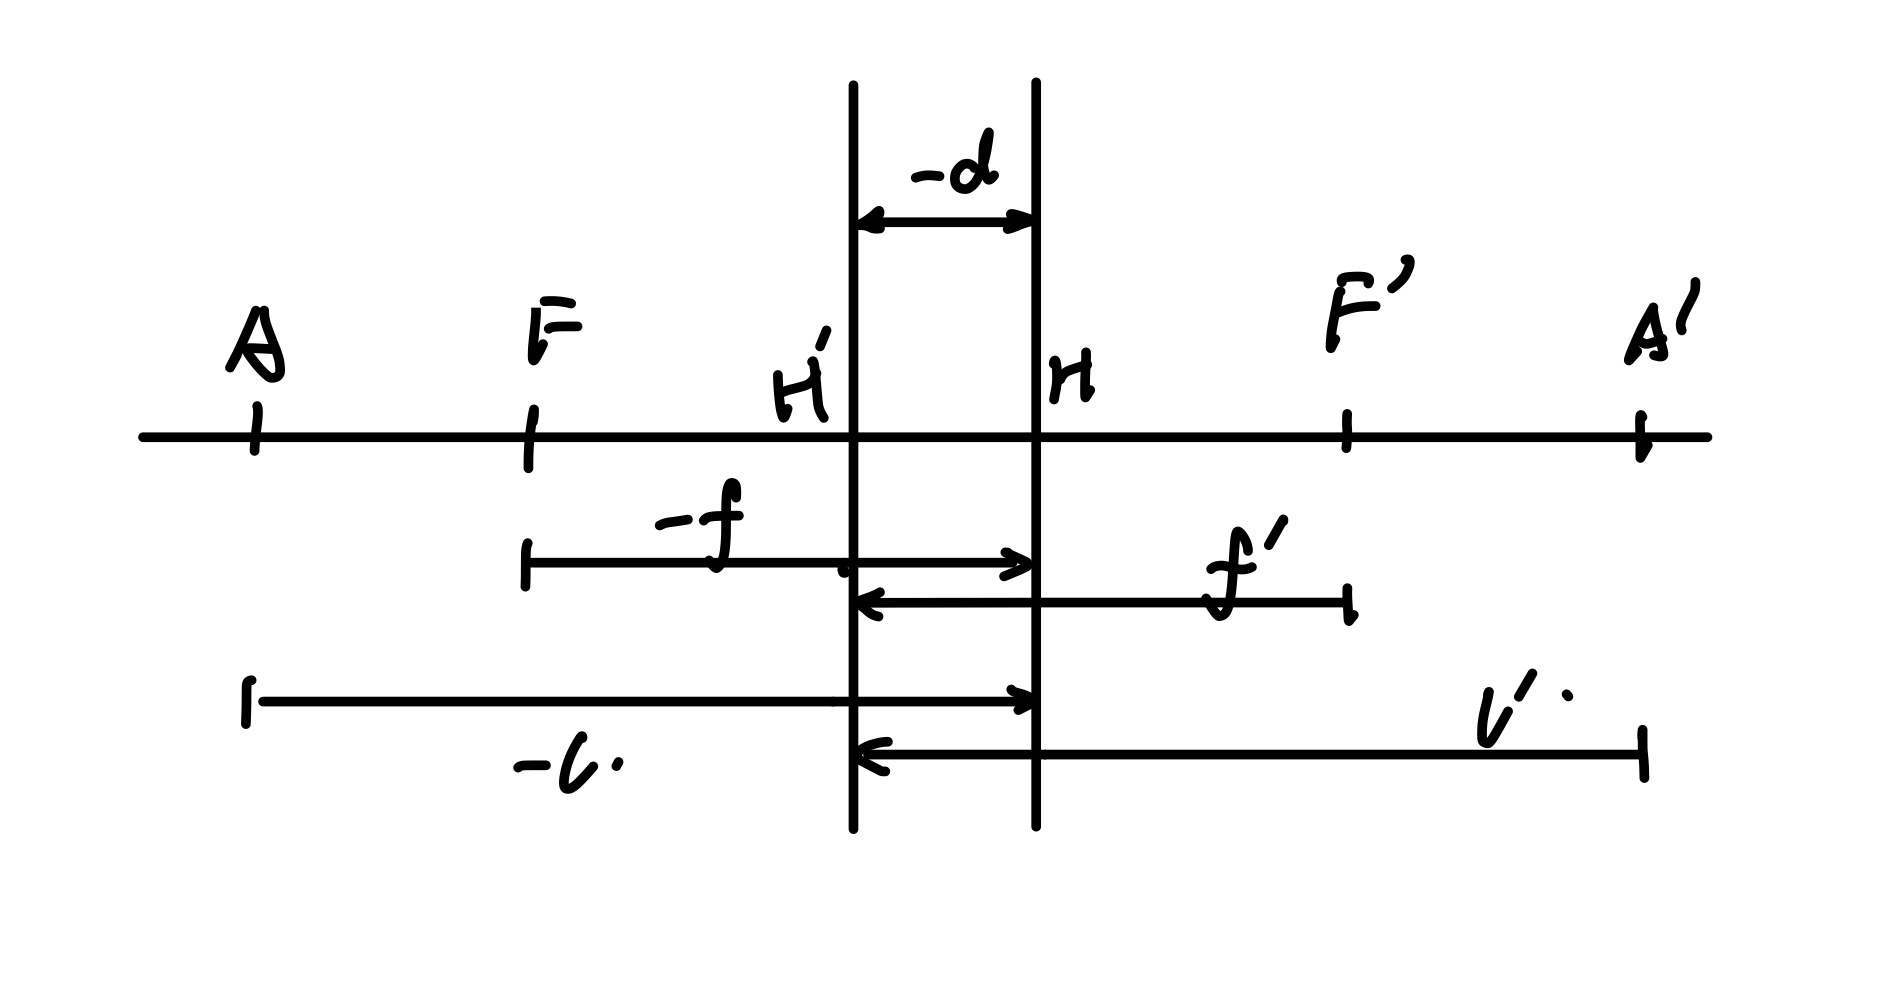
\includegraphics[width=0.5\textwidth]{image/hw2/hw2_2_2.jpeg}
    \caption{Real Base Point and Base Plane}
    \label{fig:real_base_point}
\end{figure}

\section{Problem 4}
\textbf{Chapter 2, Problem 5}\\\\

Assume the focus length of two lens are $f_1$ and $f_2$. We have.
\begin{equation}
    \begin{cases}
        \beta_1 = \frac{l'_1}{l_1}  = -1    \\
        l'_1 = l'+20                        \\
        \beta = \frac{l'}{l} = -\frac{3}{4} \\
        l1 = l
    \end{cases}
\end{equation}

Where $l_1$ and $l'_1$ are the object-side and image-side distance, $l'$,$l$ are the object-side and image-side distance of the composed system.
By solving the equation, we have
\begin{equation}
    \begin{cases}
        l_1 = -80 \\
        l_1' = 80 \\
        l = -80   \\
        l' = 60
    \end{cases}
\end{equation}

According to the composed lens equation, we have
\begin{equation}
    \frac{1}{l'_i}-\frac{1}{l_i} = \frac{1}{f_i'} = \mathit{\Phi_i}
\end{equation}

Therefore,
\begin{equation}
    \begin{cases}
        \mathit{\Phi_1} = \frac{1}{f_1'} = \frac{1}{40} \\
        \mathit{\Phi_2} = \frac{1}{f_2'} = \frac{7}{240}
    \end{cases}
\end{equation}

And for the thin lens, we have
\begin{equation}
    \mathit{\Phi} = \mathit{\Phi_1}+\mathit{\Phi_2}
\end{equation}

As a result, we have
\begin{equation}
    \mathit{\Phi_2} = \mathit{\Phi} - \mathit{\Phi_1} = \frac{1}{240}
\end{equation}

Therefore,
\begin{equation}
    \boxed{
        \begin{aligned}
            f_2' & = \frac{1}{\mathit{\Phi_2}} = 240mm \\
            f_1' & = \frac{1}{\mathit{\Phi_1}} = 40mm
        \end{aligned}
    }
\end{equation}

\section{Problem 5}
\textbf{Chapter 2, Problem 6}\\\\

Based on the Newtonian form of the lens equation, we have
\begin{align}
    xx' =   & ff'         \\
    \beta = & \frac{f}{x}
\end{align}

At the beginning, $\beta_1 = -\frac{1}{2}^{\times}$, and at the second time, $\beta_2 = -1^{\times}$. Therefore, we have
\begin{equation}
    \begin{cases}
        \beta_1 = \frac{f}{x_1} = -\frac{1}{2} \\
        \beta_2 = \frac{f}{x_2} = -1           \\
        x_1 -x_2= 100mm
    \end{cases}
\end{equation}

Solving the equation, we have
\begin{equation}
    \begin{cases}
        x_1 = 200mm \\
        x_2 = 100mm \\
    \end{cases}
\end{equation}

Therefore, the focus length of the lens is
\begin{equation}
    \boxed{
        f=100mm
    }
\end{equation}

\section{Problem 6}
\textbf{Chapter 2, Problem 7}\\\\

According to the condition, $f'>L$, therefore this is a telephoto optical group. The optical path is shown in Figure.\ref{fig:telephoto_optical_group}.
\begin{figure}[H]
    \centering
    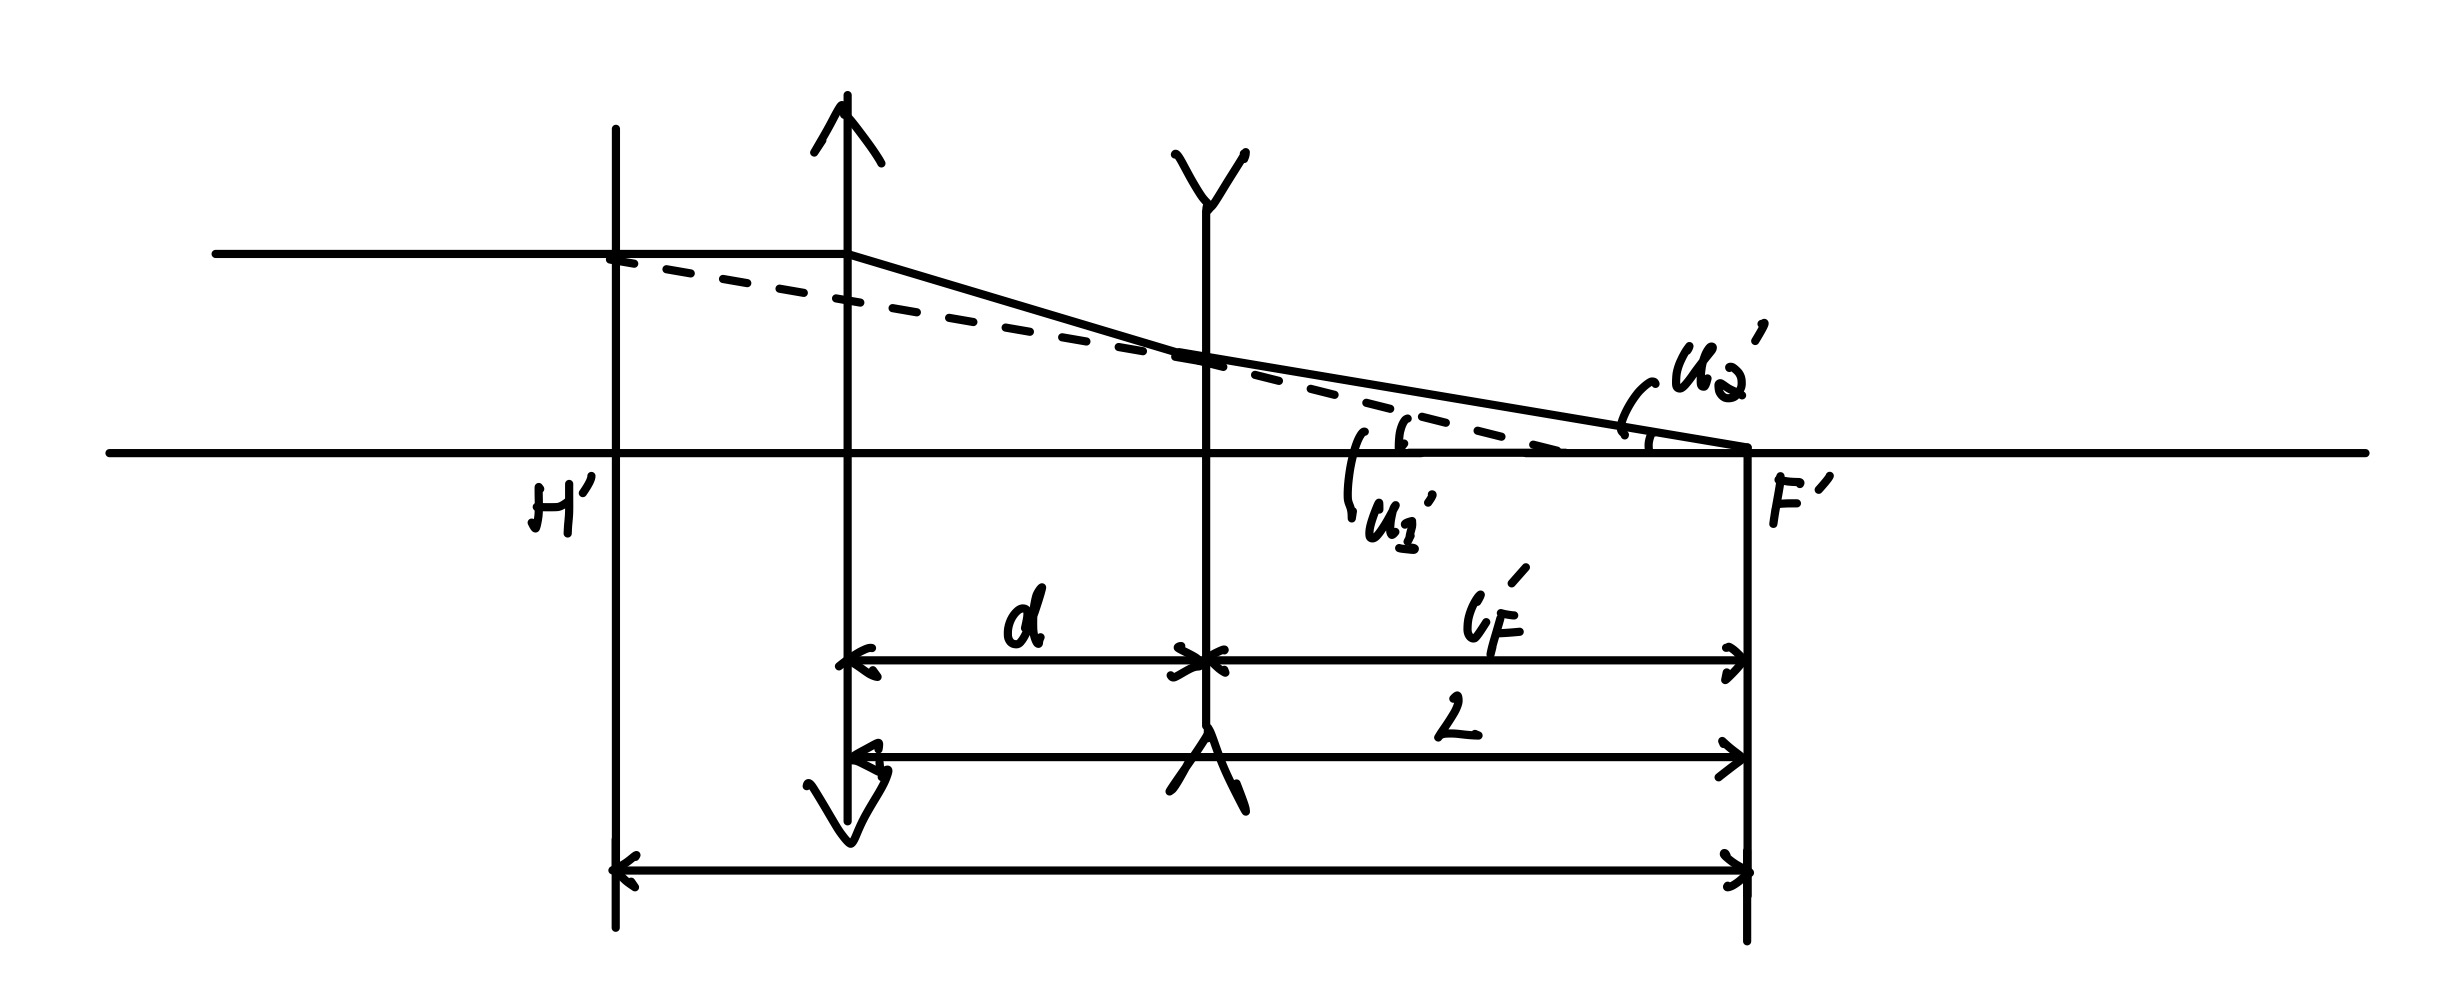
\includegraphics[width=0.5\textwidth]{image/hw2/hw2_3_1.jpeg}
    \caption{Telephoto Optical Group}
    \label{fig:telephoto_optical_group}
\end{figure}

we have,
\begin{align}
    d  & =  L-l'_F = 300mm \\
    f' & = 1200mm          \\
    l'_F = 400mm           \\
    l'_F = f'"(1-\frac{d}{f_1'})
\end{align}

Therefore,
\begin{equation}
    \boxed{
        f'_1 = \frac{d}{1-\frac{l'_F}{f'}} = \frac{300mm}{1-\frac{400}{1200}} = 450mm
    }
\end{equation}

Also we have the formula of the composed lens
\begin{equation}
    f' = -\frac{f_1'f'_2}{\Delta} = -\frac{f_1'f'_2}{d-f_1'-f'_2}
\end{equation}

So the focus length of the second lens is
\begin{equation}
    \boxed{
        f'_2 = \frac{d-f_1'}{1-\frac{f_1'}{f'}} = \frac{300mm-450mm}{1-\frac{450}{1200}} = -240mm
    }
\end{equation}

\section{Problem 7}
\textbf{Chapter 2, Problem 9}\\\\
According to the formula of lens, we have
\begin{align}
    f' =            & \frac{nr_1r_2}{(n-1)\left[n(r_2-r_1)+(n-1)d\right]}                                                     \\
    =               & \frac{1.5\cdot -200mm \cdot -300mm}{0.5\cdot \left[1.5\cdot (-300mm-(-200mm))+(1.5-1)\cdot 50mm\right]} \\
    =               & \boxed{ 600mm}                                                                                          \\
    \mathit{\Phi} = & \frac{1}{f'} = \frac{1}{600mm} = 0.001
\end{align}

\section{Problem 8}

\textbf{Chapter 2, Problem 14}\\\\
the optical path is shown in Figure.\ref{fig:optical_system_2}.
\begin{figure}[H]
    \centering
    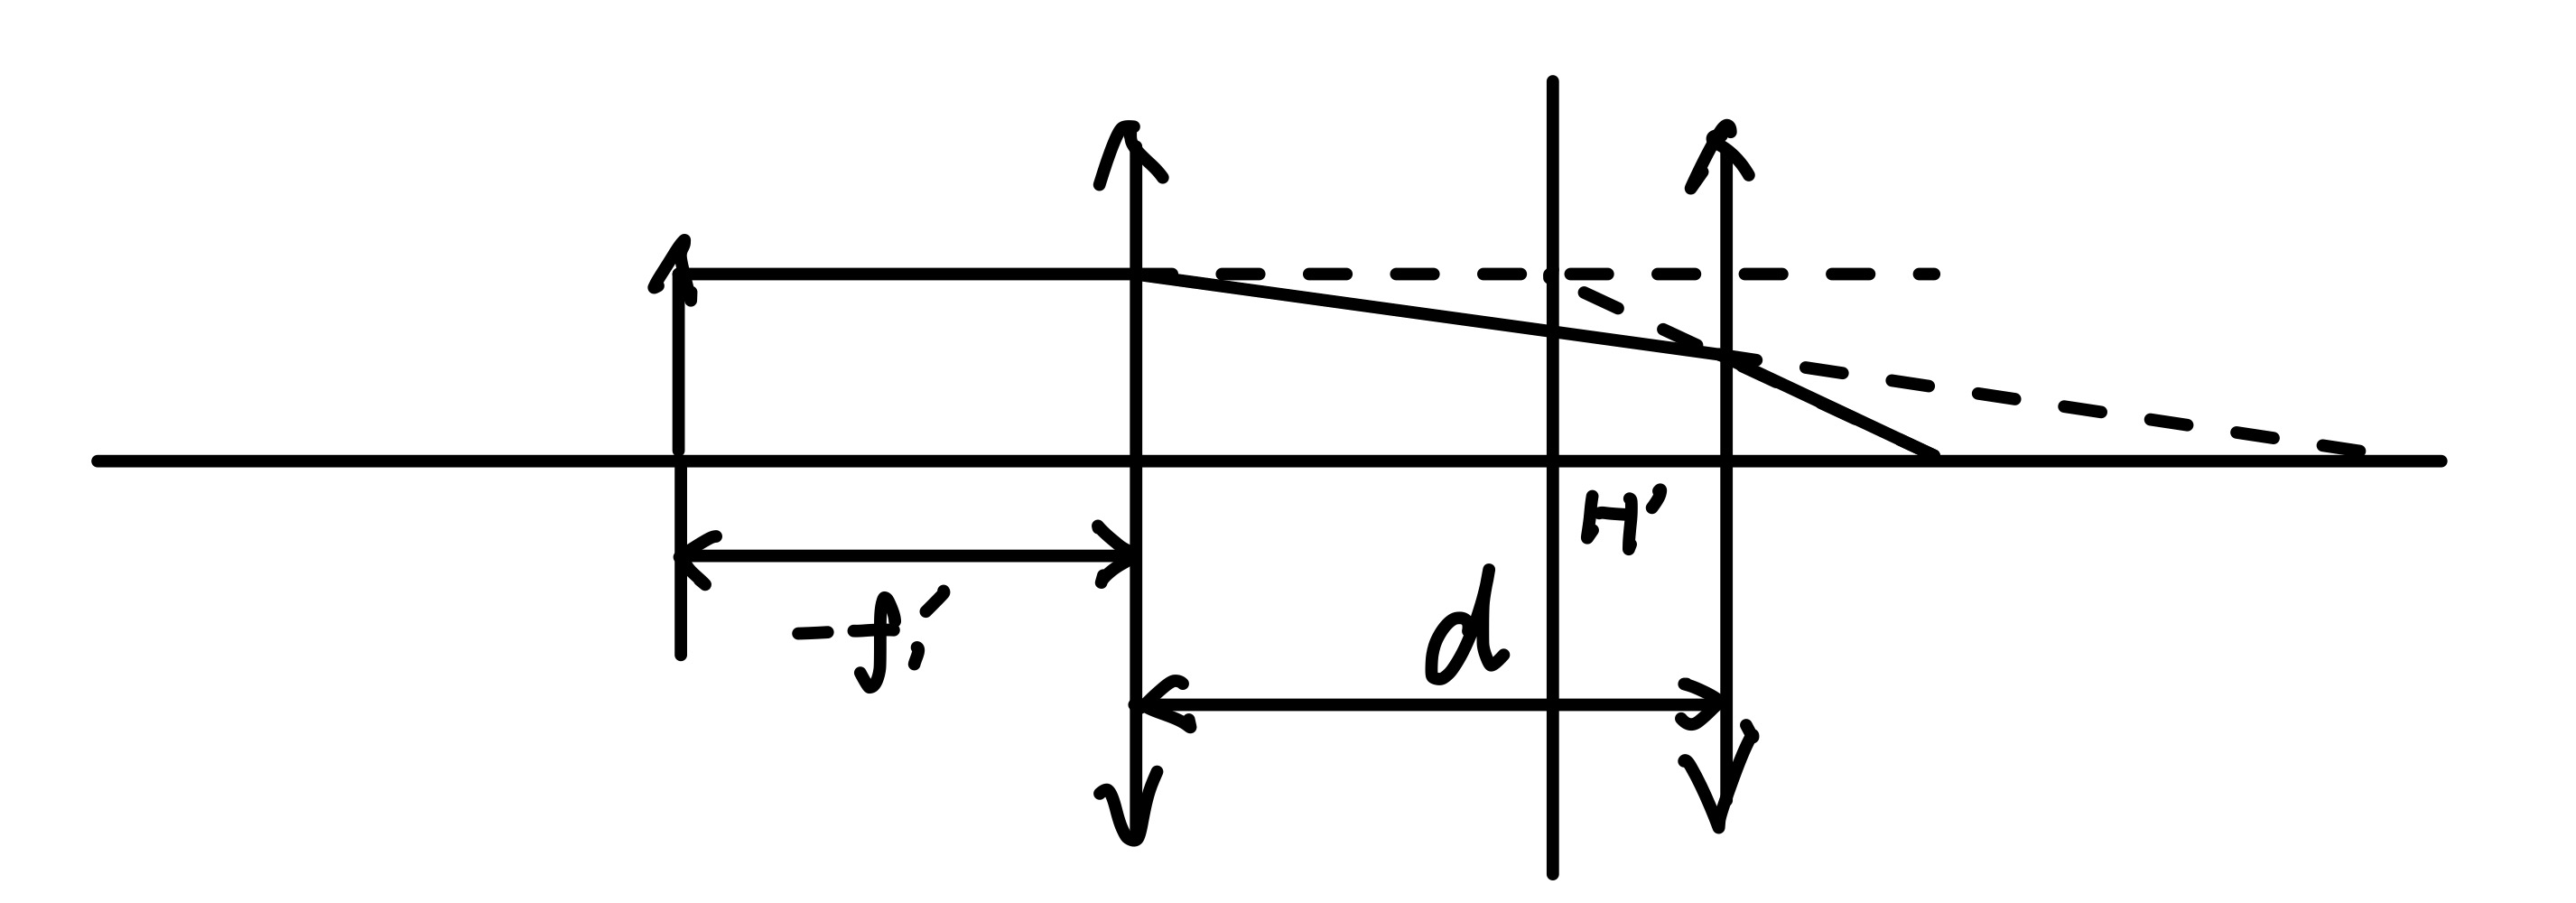
\includegraphics[width=0.5\textwidth]{image/hw2/hw2_4_1.jpeg}
    \caption{Optical System}
    \label{fig:optical_system_2}
\end{figure}

According to the condition, we have
\begin{align}
    x_F = \frac{f_1f_1'}{\Delta} = -\frac{f_1'^2}{\Delta}\\
    \Delta = d-f_1'-f_2'\\
\end{align}

Therefore, the focus length is
\begin{equation}
    f = \frac{f_1f_2}{\Delta} = \frac{f_1'f_2'}{d-f_1'-f_2'}
\end{equation}

The object is at the focus point of the first lens, so we have
\begin{equation}
    l = f-x_F\\
    l = x+f
\end{equation}

That is,
\begin{equation}
    x = -x_F = \frac{f_1'^2}{\Delta}
\end{equation}

And the vertical magnification is
\begin{equation}
    \beta = -\frac{f}{x} = -\frac{f_2'}{f_1'}
\end{equation}

\end{document}